\documentclass[xcolor=dvipsnames,10pt]{beamer}

\usetheme[presnum=03]{u18fest}

\subtitle{Marco Bayesiano para el análisis de datos,\\
  calibración de parámetros y modelamiento inverso}
\title{Teoría de Probabilidades\\
  Parte II}%
\institute{Universidad Industrial de Santander}%
\date{U18 Fest}

\usepackage{pgfplots}
\usetikzlibrary{positioning,calc}
\usepgfplotslibrary{fillbetween}
\usepackage{unicode-math}

\tikzset{%
  declare function={%
    normcdf(\x,\m,\s)=1/(1 + exp(-0.07056*((\x-\m)/\s)^3 - 1.5976*(\x-\m)/\s));%
  }%
}

\begin{document}

\begin{frame}[noframenumbering]
  \titlepage
\end{frame}

\begin{frame}
  \frametitle{Introducción}
  \begin{itemize}
  \item Cubrimos los elementos de la teoría de probabilidades
    \begin{itemize}
    \item \emph{Resultados, variables aleatorias, eventos, y probabilidades}
    \end{itemize}
  \item El modelamiento probabilístico en la práctica se basa en variables aleatorias, eventos asociados a variables aleatorias, y sus probabilidades
  \item Usualmente, la definición de espacio de resultados $\Omega$ se puede tratar de manera implícita, i.e., no es necesario definir $\Omega$ explícitamente
  \end{itemize}
\end{frame}
%
\begin{frame}
  \frametitle{Introducción}
  \emph{Ejemplo:} Altura de una población
  \begin{equation*}
    \Omega = \{ \text{personas en la población} \}
  \end{equation*}
  \begin{itemize}
  \item \textbf{Variable aleatoria}: Altura
    \begin{equation*}
      A \colon \Omega \to \mathbb{R}
    \end{equation*}
  \item \textbf{Eventos}:
    \begin{itemize}
    \item Altura mayor o igual a cierto valor $a$: $P(A \geq a)$
    \item Altura menor a cierto valor $b$: $P(A < b)$
    \end{itemize}
  \end{itemize}
  \pause
  Si el interés es en las \emph{propiedades} de la ``altura''...
  \begin{itemize}
  \item ...no es necesario pensar en $\Omega$
  \item Sólo hace falta pensar en $A$ y los valores que puede tomar
  \end{itemize}
\end{frame}
%
\begin{frame}
  \frametitle{Funciones de masa y densidad de probabilidad}
  Asocian probabilidades a los valores de variables aleatorias
  \begin{itemize}
  \item \textbf{Variables discretas}:\\
    Función de \emph{masa} de probabilidad (pmf)
  \item \textbf{Variables contínuas}:\\
    Función de \emph{densidad} acumulada (cdf)\\
    Función de \emph{densidad} de probabilidad (pdf)
  \end{itemize}
\end{frame}
%
\begin{frame}
  \frametitle{Función de masa de probabilidad (pmf)}
  \begin{itemize}
  \item \textbf{Variable aleatoria}
    \begin{equation*}
      X \colon \Omega \to C
    \end{equation*}
  \item \textbf{pmf} $p : C \to [0, 1]$ definida como
    \begin{equation*}
      p(c) = P(X = c) = P \left ( \left \{ \omega \in \Omega \colon X(\omega) = c \right \} \right )
    \end{equation*}
  \end{itemize}
\end{frame}
%
\begin{frame}
  \frametitle{Función de masa de probabilidad (pmf)}
  \emph{Ejemplo}: Lanzar dos dados.
  Suma $X \colon \Omega \to \mathbb{N}$
  \begin{columns}
    \begin{column}{0.44\textwidth}
      \begin{figure}
        \centering%
        \def\szx{0.7cm}%
        \def\szy{0.7cm}
        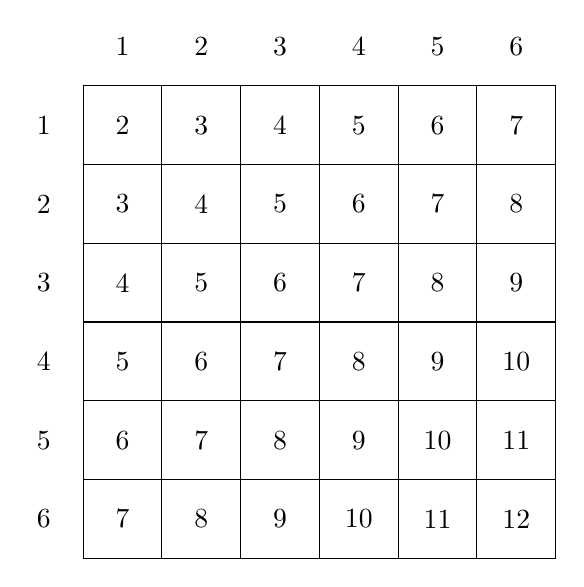
\begin{tikzpicture}
          \foreach \x in {1,...,6}{%
            \node at ($ -\x*(0,\szy) + 0.5*(0, \szy) + 0.5*(\szx, 0)$) {\x}; }%
          \foreach \y in {1,...,6}{%
            \node at ($ \y*(\szx,0) + 0.5*(0, \szy) + 0.5*(\szx, 0)$) {\y}; }%
          \foreach \x in {1,...,6}{%
            \foreach \y in {1,...,6}{%
              \pgfmathsetmacro\z{int(\x+\y)}%
              \draw ($ -\x*(0,\szy) + \y*(\szx,0) $) rectangle+(\szx,\szy);%
              \node at ($ -\x*(0,\szy) + \y*(\szx,0) + 0.5*(\szx, \szy)$) {\z};%
            }%
          }
        \end{tikzpicture}
      \end{figure}
    \end{column}
    \begin{column}{0.52\textwidth}
      \vskip2em
      \textbf{pmf}:
      \begin{overprint}
        \onslide<1>
        \begin{itemize}
        \item $p(1) = 0$
        \item $p(2) = 1 / 36$
        \item $p(3) = 2 / 36$
        \item $p(4) = 3 / 36$\\
          $\dots$
        \end{itemize}
        \onslide<2->
        \begin{figure}
          \centering
          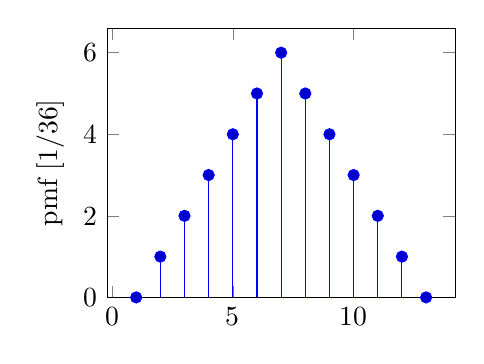
\begin{tikzpicture}
            \begin{axis}[ymin=0, height=5cm, width=6cm, ylabel={pmf $[1 / 36]$}, ylabel near ticks]
              \addplot+ [ycomb] coordinates {%
                (1, 0) (2, 1) (3, 2) (4, 3) (5, 4) (6, 5) (7, 6) (8, 5) (9, 4) (10, 3) (11, 2) (12, 1) (13, 0)%
              };
            \end{axis}
          \end{tikzpicture}
        \end{figure}
      \end{overprint}
    \end{column}
  \end{columns}
\end{frame}
%
\begin{frame}
  \frametitle{Función de masa de probabilidad (pmf)}
  \begin{itemize}
  \item Para la variable aleatoria discreta $X \colon \Omega \to C$, se puede utilizar la pmf para calcular la probabilidad del evento del valor de $X$ estar en cualquier subconjunto $B \subseteq C$:
    \begin{equation*}
      P(X \in B) = \sum_{b \in B} p(b)
    \end{equation*}
    \pause
  \item Como consecuencia,
    \begin{equation*}
      \sum_{b \in C} p(b) = 1
    \end{equation*}
  \item \textbf{Ejemplo}: Lanzar dos dados
    \begin{equation*}
      p(1) + p(2) + p(3) + \dots + p(11) + p(12) + \dots = 1
    \end{equation*}
  \end{itemize}
\end{frame}
%
\begin{frame}
  \frametitle{Muestrear variables aleatorias}
  \begin{itemize}
  \item Vamos a usar \emph{generadores de números pseudo-aleatorios} (PRNGs)
  \item PRNGs \textbf{no} generan números realmente aleatorios...
  \item ...pero generan una secuencia de números con propiedades aproximadamente iguales a las propiedades de secuencias de números aleatorios
  \item La secuencia de un PRNG es determinada por un valor inicial llamdo \emph{semilla} (seed)
  \item Dada la misma semilla, un cierto PRNG genera la misma secuencia cada vez que es invocado
  \end{itemize}
\end{frame}
%
\begin{frame}
  \frametitle{Función de densidad acumulada (cdf)}
  \begin{itemize}
  \item \textbf{Variable aleatoria}
    \begin{equation*}
      X \colon \Omega \to C
    \end{equation*}
  \item \textbf{cdf} $F(c) = P(X \leq c) \in [0, 1]$
    \pause
  \item \textbf{Ejemplo}: Variable aleatoria normal estándar
    \vskip1em
    \begin{figure}
      \centering
      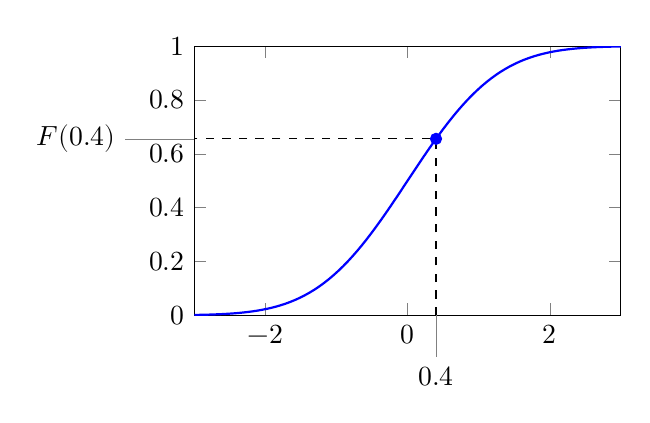
\begin{tikzpicture}
        \pgfmathsetmacro\myextraytick{normcdf(0.4, 0, 1)}%
        \begin{axis}[ymin=0, ymax=1, xmin=-3, xmax=3, height=5cm, width=7cm, %
          extra tick style={%
            tick align=outside, tick pos=left, grid style={dotted,black}%
          }, %
          extra x tick style={%
            major tick length=1.25\baselineskip%
          }, %
          extra y tick style={%
            major tick length=2.5em%
          }, %
          extra x ticks={0.4}, extra x tick labels={$0.4$}, extra y ticks={\myextraytick}, extra y tick labels={$F(0.4)$}]
          \addplot [samples=150, no markers, blue, thick] {normcdf(x, 0, 1)};%
          \addplot[mark=*,color=blue] coordinates {(0.4, {normcdf(0.4, 0, 1)})};%
          \draw [dashed] (axis cs: 0.4, 0.0) |- (axis cs: -3, {normcdf(0.4, 0, 1)});%
        \end{axis}
      \end{tikzpicture}
    \end{figure}
  \end{itemize}
\end{frame}
%
\begin{frame}
  \frametitle{Función de densidad cumulativa}
  \begin{figure}
    \centering
    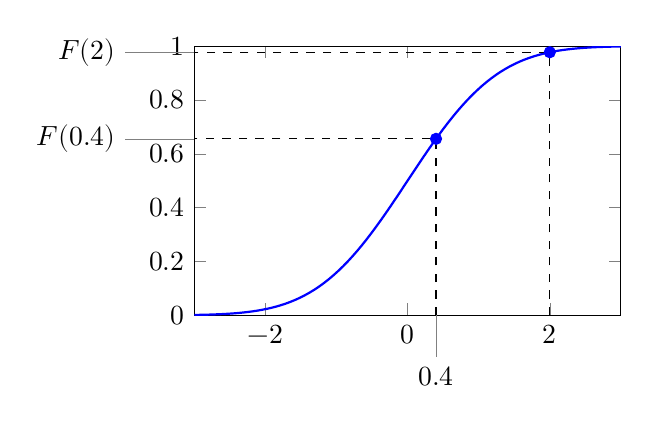
\begin{tikzpicture}
      \pgfmathsetmacro\myextrayticka{normcdf(0.4, 0, 1)}%
      \pgfmathsetmacro\myextraytickb{normcdf(2.0, 0, 1)}%
      \begin{axis}[ymin=0, ymax=1, xmin=-3, xmax=3, height=5cm, width=7cm, %
        extra tick style={%
          tick align=outside, tick pos=left, grid style={dotted,black}%
        }, %
        extra x tick style={%
          major tick length=1.25\baselineskip%
        }, %
        extra y tick style={%
          major tick length=2.5em%
        }, %
        extra x ticks={0.4}, extra x tick labels={$0.4$}, extra y ticks={\myextrayticka, \myextraytickb}, extra y tick labels={$F(0.4)$, $F(2)$}]
        \addplot [samples=150, no markers, blue, thick] {normcdf(x, 0, 1)};%
        \addplot[mark=*,color=blue] coordinates {(0.4, {normcdf(0.4, 0, 1)})};%
        \draw [dashed] (axis cs: 0.4, 0.0) |- (axis cs: -3, {normcdf(0.4, 0, 1)});%
        \addplot[mark=*,color=blue] coordinates {(2.0, {normcdf(2.0, 0, 1)})};%
        \draw [dashed] (axis cs: 2.0, 0.0) |- (axis cs: -3, {normcdf(2.0, 0, 1)});
      \end{axis}
    \end{tikzpicture}
  \end{figure}
  La cdf puede utilizarse para evaluar la probabilidad de varios escenarios:
  \begin{itemize}
  \item $P(X > 2) = 1 - P(X \leq 2) = 1 - F(2)$
  \item $P(0.4 \leq X \leq 2) = P(X \leq 2) - P(X \leq 0.4) = F(2) - F(0.4)$
  \end{itemize}
\end{frame}
%
\begin{frame}
  \frametitle{Variables aleatorias contínuas}
  \begin{itemize}
  \item La cdf no es la equivalente de la pmf para variables aleatorias contínuas
    \begin{itemize}
    \item La pmf asigna probabilidades a valores individuales
    \item La cdf asigna probabilidades a \emph{intervalos} de valores
    \end{itemize}
  \item Para generalizar la pmf debemos utilizar el concepto de \emph{densidad}
  \end{itemize}
\end{frame}
%
\begin{frame}
  \frametitle{Función de densidad de probabilidad (pdf)}
  La pdf (o \emph{densidad}) $p(a)$ cuantifica la cantidad de probabilidad en un intervalo alrededor de $a$ relativa a la longitud del intervalo%
  \vskip1em
  \emph{Ejemplo}: Variable aleatoria normal estándar
  \begin{overprint}
    \onslide<1>
    \begin{figure}
      \centering
      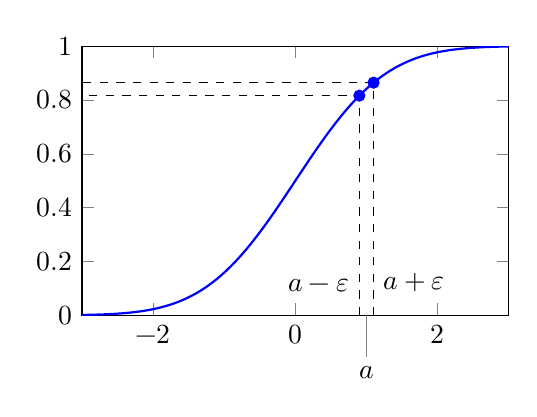
\begin{tikzpicture}
        \pgfmathsetmacro\myextrayticka{normcdf(0.9, 0, 1)}%
        \pgfmathsetmacro\myextraytickb{normcdf(1.1, 0, 1)}%
        \begin{axis}[ymin=0, ymax=1, xmin=-3, xmax=3, height=5cm, width=7cm, %
          extra tick style={%
            tick align=outside, tick pos=left, grid style={dotted,black}%
          }, %
          extra x tick style={%
            major tick length=1.25\baselineskip%
          }, %
          extra y tick style={%
            major tick length=2.5em%
          }, %
          extra x ticks={1.0}, extra x tick labels={$a$}]
          \addplot [samples=150, no markers, blue, thick] {normcdf(x, 0, 1)};%
          \addplot[mark=*,color=blue] coordinates {(0.9, {normcdf(0.9, 0, 1)})};%
          \draw [dashed] (axis cs: 0.9, 0.0) |- (axis cs: -3, {normcdf(0.9, 0, 1)});%
          \addplot[mark=*,color=blue] coordinates {(1.1, {normcdf(1.1, 0, 1)})};%
          \draw [dashed] (axis cs: 1.1, 0.0) |- (axis cs: -3, {normcdf(1.1, 0, 1)});%
          \node at (axis cs: 0.9, 0.05) [anchor=south east] {$a - \varepsilon$};%
          \node at (axis cs: 1.1, 0.05) [anchor=south west] {$a + \varepsilon$};
        \end{axis}
      \end{tikzpicture}
    \end{figure}
    \onslide<2->
    \begin{figure}
      \centering
      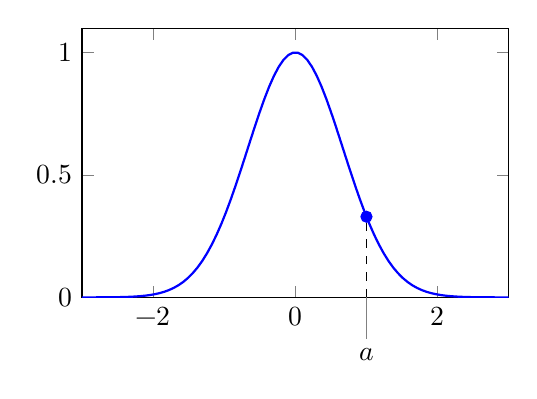
\begin{tikzpicture}
        \begin{axis}[ymin=0, xmin=-3, xmax=3, height=5cm, width=7cm, %
          extra tick style={%
            tick align=outside, tick pos=left, grid style={dotted,black}%
          }, %
          extra x tick style={%
            major tick length=1.25\baselineskip%
          }, %
          extra y tick style={%
            major tick length=2.5em%
          }, %
          extra x ticks={1.0}, extra x tick labels={$a$}]
          \addplot [samples=150, no markers, blue, thick] {exp{-0.5*x^2}/sqrt{2*pi}};%
          \addplot[mark=*,color=blue] coordinates {(1.0, exp{-0.5}/sqrt{2*pi})};%
          \draw [dashed] (axis cs: 1.0, 0.0) -- (axis cs: 1.0, exp{-0.5}/sqrt{2*pi});%
        \end{axis}
      \end{tikzpicture}
    \end{figure}
  \end{overprint}
\end{frame}
%
\begin{frame}
  \frametitle{Función de densidad de probabilidad (pdf)}

  \begin{itemize}
  \item Para la variable aleatoria $X \colon \Omega \to C$, la pdf y la cdf están conectadas a través de la relación
    \begin{equation*}
      F(a) = P(X \leq a) = \int^a_{-\infty} p(x) \, \symrm{d} x
    \end{equation*}
    Qué quiere decir ésto?\pause
  \item Si quiero calcular la probabilidad del evento ${\infty \leq X \leq a}$, basta con ``integrar'' la densidad sobre el intervalo $(-\infty, a]$
  \item Podemos generalizar ésta relación para calcular la probabilidad del evento del valor de $X$ estar en cualquier subconjunto $B \subseteq C$:
    \begin{equation*}
      P(X \in B) = \int_B p(x) \, \symrm{d} x
    \end{equation*}
  \item Como consecuencia,
    \begin{equation*}
      P(X \in C) = \int_C p(x) \, \symrm{d} x = 1
    \end{equation*}
  \end{itemize}
\end{frame}
%
\begin{frame}
  \frametitle{Función de densidad de probabilidad (pdf)}
  \begin{itemize}
  \item Para variables aleatorias \emph{discretas},
    \begin{equation*}
      P(X \in B) = \sum_{b \in B } p(b)
    \end{equation*}
  \item Para variables aleatorias \emph{contínuas},
    \begin{equation*}
      P(X \in B) = \int_B p(x) \, \symrm{d} x
    \end{equation*}
  \item La pdf generaliza la pmf a variables aleatorias contínuas
  \item La integral $\int$ generaliza la suma $\sum$ a variables aleatorias contínuas
  \end{itemize}
\end{frame}
%
\begin{frame}
  \frametitle{Función de densidad de probabilidad (pdf)}
  \begin{itemize}
  \item La integral $\int_B p(x) \, \symrm{d} x$ puede interpretarse como el área bajo la curva $y = p(x)$ en el intervalo $B$
  \item E.g., para el intervalo $B = (a, b)$,
    \vskip1em
    \begin{figure}
      \centering
      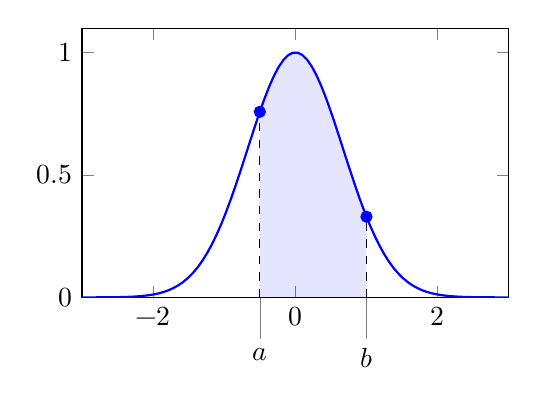
\begin{tikzpicture}
        \begin{axis}[ymin=0, xmin=-3, xmax=3, height=5cm, width=7cm, %
          extra tick style={%
            tick align=outside, tick pos=left, grid style={dotted,black}%
          }, %
          extra x tick style={%
            major tick length=1.25\baselineskip%
          }, %
          extra y tick style={%
            major tick length=2.5em%
          }, %
          extra x ticks={-0.5, 1.0}, extra x tick labels={$a$, $b$}]
          \addplot [name path=f, samples=150, no markers, blue, thick] {exp{-0.5*x^2}/sqrt{2*pi}};%
          \path[name path=axis] (axis cs:-0.5,0) -- (axis cs:1.0,0);%
          \addplot [thick, color=blue, fill=blue, fill opacity=0.1] fill between [of=f and axis, soft clip={domain=-0.5:1.0}];
          %
          \addplot[mark=*,color=blue] coordinates {(-0.5, exp{-0.125}/sqrt{2*pi})};%
          \draw [dashed] (axis cs: -0.5, 0.0) -- (axis cs: -0.5, exp{-0.125}/sqrt{2*pi});%
          %
          \addplot[mark=*,color=blue] coordinates {(1.0, exp{-0.5}/sqrt{2*pi})};%
          \draw [dashed] (axis cs: 1.0, 0.0) -- (axis cs: 1.0, exp{-0.5}/sqrt{2*pi});%
        \end{axis}
      \end{tikzpicture}
    \end{figure}
  \item Dado que $\int_C p(x) \, \mathrm{d} x = 1$, eso indica que el área bajo la pdf es $1$
  \item La cdf $F(a)$ corresponde al área bajo la curva entre $-\infty$ y $a$
  \end{itemize}
\end{frame}
%
\begin{frame}
  \frametitle{Ejemplo}
  \begin{itemize}
  \item Variable aleatoria normal estándar $X \sim \mathcal{N}(0, 1)$
  \item Para un valor $\alpha \in [0, 1]$,  hay un intervalo $B = (a, b)$ para el cual
    \begin{itemize}
    \item $p(a) = p(b)$
    \item $P(X \in B) = 1 - \alpha$
    \end{itemize}
  \item 
  \end{itemize}
\end{frame}

\end{document}

%%% Local Variables:
%%% TeX-master: t
%%% TeX-engine: luatex
%%% ispell-local-dictionary: "spanish"
%%% End:
